% Topic 3.4: Bitcoin vs. Ethereum
% Self-contained Beamer presentation (40 slides)
\documentclass[11pt,aspectratio=169]{beamer}
\usetheme{Madrid}

% ======================= PACKAGES =======================
\usepackage{graphicx}
\usepackage{booktabs}
\usepackage{adjustbox}
\usepackage{multicol}
\usepackage{amsmath}
\usepackage{amssymb}
\usepackage{tikz}
\usetikzlibrary{arrows,shapes,positioning,shadows,trees}
\usepackage{listings}
\usepackage{xcolor}

% ======================= COLOR DEFINITIONS =======================
% Primary color scheme: Blue/Teal for Digital Finance
\definecolor{dfblue}{RGB}{0,102,204}
\definecolor{dfteal}{RGB}{0,153,153}
\definecolor{dfcyan}{RGB}{51,187,204}
\definecolor{dflightblue}{RGB}{153,204,255}
\definecolor{dflightblue2}{RGB}{173,214,255}
\definecolor{dflightblue3}{RGB}{193,224,255}
\definecolor{dflightblue4}{RGB}{213,234,255}

% Accent colors for finance applications
\definecolor{dfgreen}{RGB}{44, 160, 44}
\definecolor{dfred}{RGB}{214, 39, 40}
\definecolor{dforange}{RGB}{255, 127, 14}
\definecolor{dfgray}{RGB}{127, 127, 127}

% Utility colors
\definecolor{lightgray}{RGB}{240, 240, 240}
\definecolor{midgray}{RGB}{180, 180, 180}
\definecolor{codebg}{RGB}{245, 245, 245}

% ======================= THEME CUSTOMIZATION =======================
% Apply Digital Finance color scheme to Madrid theme
\setbeamercolor{palette primary}{bg=dflightblue3,fg=dfblue}
\setbeamercolor{palette secondary}{bg=dflightblue2,fg=dfblue}
\setbeamercolor{palette tertiary}{bg=dfteal,fg=white}
\setbeamercolor{palette quaternary}{bg=dfblue,fg=white}

\setbeamercolor{structure}{fg=dfblue}
\setbeamercolor{section in toc}{fg=dfblue}
\setbeamercolor{subsection in toc}{fg=dfteal}
\setbeamercolor{title}{fg=dfblue}
\setbeamercolor{frametitle}{fg=dfblue,bg=dflightblue3}
\setbeamercolor{block title}{bg=dflightblue2,fg=dfblue}
\setbeamercolor{block body}{bg=dflightblue4,fg=black}

% Remove navigation symbols for cleaner look
\setbeamertemplate{navigation symbols}{}

% Clean itemize/enumerate
\setbeamertemplate{itemize items}[circle]
\setbeamertemplate{enumerate items}[default]

% Margins for readability
\setbeamersize{text margin left=8mm,text margin right=8mm}

% ======================= LISTINGS CONFIGURATION =======================
% Python code style
\lstdefinestyle{pythonstyle}{
    language=Python,
    basicstyle=\ttfamily\footnotesize,
    keywordstyle=\color{dfblue}\bfseries,
    stringstyle=\color{dforange},
    commentstyle=\color{dfgray}\itshape,
    numberstyle=\tiny\color{dfgray},
    numbers=left,
    numbersep=5pt,
    backgroundcolor=\color{codebg},
    showspaces=false,
    showstringspaces=false,
    showtabs=false,
    frame=single,
    rulecolor=\color{midgray},
    tabsize=4,
    captionpos=b,
    breaklines=true,
    breakatwhitespace=false,
    escapeinside={(*@}{@*)},
    xleftmargin=10pt,
    xrightmargin=10pt
}

% Solidity code style
\lstdefinestyle{soliditystyle}{
    language=Java, % closest approximation
    basicstyle=\ttfamily\footnotesize,
    keywordstyle=\color{dfteal}\bfseries,
    stringstyle=\color{dforange},
    commentstyle=\color{dfgray}\itshape,
    numberstyle=\tiny\color{dfgray},
    numbers=left,
    numbersep=5pt,
    backgroundcolor=\color{codebg},
    showspaces=false,
    showstringspaces=false,
    showtabs=false,
    frame=single,
    rulecolor=\color{midgray},
    tabsize=2,
    captionpos=b,
    breaklines=true,
    breakatwhitespace=false,
    escapeinside={(*@}{@*)},
    xleftmargin=10pt,
    xrightmargin=10pt,
    morekeywords={pragma, contract, function, returns, public, private, view, pure, payable, address, uint256, mapping, event, modifier}
}

% Inline code command
\newcommand{\code}[1]{\texttt{\color{dfblue}#1}}

% ======================= CUSTOM COMMANDS =======================
% Bottom annotation (Madrid-style)
\newcommand{\bottomnote}[1]{%
\vfill
\vspace{-2mm}
\textcolor{dflightblue2}{\rule{\textwidth}{0.4pt}}
\vspace{1mm}
\footnotesize
\textbf{#1}
}

% Compact list spacing
\newcommand{\compactlist}{%
\setlength{\itemsep}{0pt}%
\setlength{\parskip}{0pt}%
\setlength{\parsep}{0pt}%
}

% Chart placeholder
\newcommand{\chartplaceholder}[2][5cm]{%
\begin{center}
\begin{adjustbox}{max width=0.95\textwidth, max height=#1}
\framebox[\textwidth][c]{%
\rule{0pt}{#1}%
\textcolor{midgray}{[#2]}%
}
\end{adjustbox}
\end{center}
}

% ======================= FINANCE NOTATION MACROS =======================
% Probability and statistics
\newcommand{\E}{\mathbb{E}} % Expected value
\newcommand{\Var}{\mathrm{Var}} % Variance
\newcommand{\Cov}{\mathrm{Cov}} % Covariance
\newcommand{\Prob}{\mathbb{P}} % Probability

% Distributions
\newcommand{\Normal}{\mathcal{N}} % Normal distribution
\newcommand{\Uniform}{\mathcal{U}} % Uniform distribution

% Returns and prices
\newcommand{\Ret}{R} % Return
\newcommand{\LogRet}{r} % Log return
\newcommand{\Price}{S} % Price/Stock price
\newcommand{\Strike}{K} % Strike price

% Options and derivatives
\newcommand{\CallPrice}{C} % Call option price
\newcommand{\PutPrice}{P} % Put option price
\newcommand{\Greeks}[1]{\mathit{#1}} % Greek letters

% Risk measures
\newcommand{\VaR}{\mathrm{VaR}} % Value at Risk
\newcommand{\CVaR}{\mathrm{CVaR}} % Conditional VaR
\newcommand{\Sharpe}{\mathrm{SR}} % Sharpe Ratio

% Time series
\newcommand{\AR}{\mathrm{AR}} % Autoregressive
\newcommand{\MA}{\mathrm{MA}} % Moving average
\newcommand{\GARCH}{\mathrm{GARCH}} % GARCH

% Blockchain/Crypto
\newcommand{\Hash}{\mathrm{Hash}} % Hash function
\newcommand{\Block}{\mathcal{B}} % Block
\newcommand{\Chain}{\mathcal{C}} % Chain

% Real numbers, integers
\newcommand{\R}{\mathbb{R}}
\newcommand{\Z}{\mathbb{Z}}
\newcommand{\N}{\mathbb{N}}

% ======================= TIKZ STYLES =======================
% Styles for finance-related diagrams
\tikzstyle{process} = [rectangle, minimum width=3cm, minimum height=1cm, text centered, draw=dfblue, fill=dflightblue4, thick]
\tikzstyle{decision} = [diamond, minimum width=3cm, minimum height=1cm, text centered, draw=dfteal, fill=dflightblue4, thick]
\tikzstyle{arrow} = [thick,->,>=stealth,color=dfblue]
\tikzstyle{blockchain} = [rectangle, rounded corners, minimum width=2.5cm, minimum height=1cm, text centered, draw=dfteal, fill=dflightblue3, thick]
\tikzstyle{transaction} = [circle, minimum size=0.8cm, text centered, draw=dforange, fill=dflightblue4, thick]

% ======================= FOOTER TEMPLATE =======================
\setbeamertemplate{footline}{
    \hbox{\begin{beamercolorbox}[wd=\paperwidth,ht=2.5ex,dp=1ex,leftskip=.5em,rightskip=.5em]{author in head/foot}
    \tiny
    \textbf{Digital Finance} \hfill
    Joerg Osterrieder \hfill
    \insertdate \hfill
    Page \insertframenumber{} / \inserttotalframenumber
    \end{beamercolorbox}}
}

% ======================= SECTION DIVIDER TEMPLATE =======================
\AtBeginSection[]{
\begin{frame}[plain]
\vfill
\centering
\begin{beamercolorbox}[sep=12pt,center]{title}
\usebeamerfont{title}\LARGE\insertsection\par
\end{beamercolorbox}
\vfill
\end{frame}
}


\title{Topic 3.4: Bitcoin vs. Ethereum}
\subtitle{Two Design Philosophies}
\author{Joerg Osterrieder}
\institute{Digital Finance}
\date{2025}

\begin{document}

% =============================================================================
% SLIDE 1: Title
% =============================================================================
\begin{frame}
\titlepage
\end{frame}

% =============================================================================
% SLIDE 2: Learning Objectives
% =============================================================================
\begin{frame}{Learning Objectives}
After completing this topic, you will be able to:

\begin{enumerate}
\item \textbf{Compare} the fundamental design philosophies of Bitcoin and Ethereum

\vspace{2mm}
\item \textbf{Explain} the technical differences: consensus, scripting, and supply models

\vspace{2mm}
\item \textbf{Define} what smart contracts are and why they matter

\vspace{2mm}
\item \textbf{Analyze} the security vs. flexibility tradeoff in blockchain design

\vspace{2mm}
\item \textbf{Evaluate} which platform suits different use cases
\end{enumerate}

\vspace{5mm}
\begin{block}{Key Insight}
Bitcoin and Ethereum are not competitors -- they are different tools designed for different jobs.
\end{block}
\end{frame}

% =============================================================================
% SLIDES 3-4: Prerequisites/Background
% =============================================================================
\begin{frame}{Prerequisites: Blockchain Fundamentals Recap}
\textbf{From Topic 3.2, recall:}

\begin{columns}[T]
\begin{column}{0.48\textwidth}
\textbf{What is a Blockchain?}
\begin{itemize}\compactlist
\item Distributed ledger of transactions
\item Blocks linked by cryptographic hashes
\item No central authority
\item Immutable record (hard to change)
\end{itemize}
\end{column}
\begin{column}{0.48\textwidth}
\textbf{Key Components}
\begin{itemize}\compactlist
\item \textbf{Nodes:} Computers running the network
\item \textbf{Consensus:} How nodes agree on truth
\item \textbf{Transactions:} Records of value transfer
\item \textbf{Blocks:} Groups of transactions
\end{itemize}
\end{column}
\end{columns}

\vspace{5mm}
\begin{center}
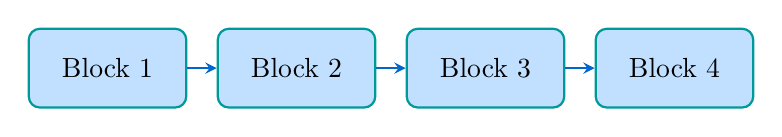
\begin{tikzpicture}[scale=0.8]
\node[blockchain, minimum width=2cm] (b1) at (0,0) {Block 1};
\node[blockchain, minimum width=2cm] (b2) at (3,0) {Block 2};
\node[blockchain, minimum width=2cm] (b3) at (6,0) {Block 3};
\node[blockchain, minimum width=2cm] (b4) at (9,0) {Block 4};

\draw[arrow] (b1) -- (b2);
\draw[arrow] (b2) -- (b3);
\draw[arrow] (b3) -- (b4);
\end{tikzpicture}
\end{center}
\end{frame}

\begin{frame}{Prerequisites: Consensus Mechanisms}
\textbf{How do blockchains agree on the ``truth''?}

\vspace{3mm}
\begin{columns}[T]
\begin{column}{0.48\textwidth}
\textbf{Proof of Work (PoW)}
\begin{itemize}\compactlist
\item Miners solve computational puzzles
\item First to solve adds the block
\item Requires significant energy
\item Security through computational cost
\item Example: Bitcoin
\end{itemize}
\end{column}
\begin{column}{0.48\textwidth}
\textbf{Proof of Stake (PoS)}
\begin{itemize}\compactlist
\item Validators lock up cryptocurrency
\item Selected based on stake amount
\item Energy efficient
\item Security through economic incentives
\item Example: Ethereum (since 2022)
\end{itemize}
\end{column}
\end{columns}

\vspace{5mm}
\begin{block}{The Blockchain Trilemma}
Every blockchain must balance three properties:
\begin{center}
\textbf{Decentralization} -- \textbf{Security} -- \textbf{Scalability}
\end{center}
You cannot maximize all three simultaneously.
\end{block}
\end{frame}

% =============================================================================
% SLIDES 5-24: Core Content
% =============================================================================
\begin{frame}{Two Visions of Blockchain}
\begin{columns}[T]
\begin{column}{0.48\textwidth}
\begin{center}
\textbf{\Large Bitcoin}\\[2mm]
\textit{``Digital Gold''}
\end{center}

\vspace{3mm}
\begin{itemize}\compactlist
\item Store of value
\item Fixed supply (21M)
\item Minimal, robust
\item Conservative changes
\item ``Don't break what works''
\end{itemize}

\vspace{3mm}
\begin{center}
\fbox{\parbox{0.85\textwidth}{\centering
\textbf{Goal:} Sound money that\\no one can inflate or censor
}}
\end{center}
\end{column}
\begin{column}{0.48\textwidth}
\begin{center}
\textbf{\Large Ethereum}\\[2mm]
\textit{``World Computer''}
\end{center}

\vspace{3mm}
\begin{itemize}\compactlist
\item Platform for applications
\item Programmable money
\item Feature-rich, flexible
\item Active development
\item ``Move fast, iterate''
\end{itemize}

\vspace{3mm}
\begin{center}
\fbox{\parbox{0.85\textwidth}{\centering
\textbf{Goal:} Decentralized platform\\for any application
}}
\end{center}
\end{column}
\end{columns}
\end{frame}

\begin{frame}{Historical Context}
\begin{center}
\begin{tabular}{c|l}
\textbf{Year} & \textbf{Event} \\
\hline
2009 & Bitcoin launches (Satoshi Nakamoto) \\
2012 & Colored coins on Bitcoin (limited tokens) \\
2013 & Ethereum whitepaper (Vitalik Buterin) \\
2015 & Ethereum launches \\
2022 & Ethereum transitions to Proof of Stake \\
\end{tabular}
\end{center}

\vspace{5mm}
\textbf{Vitalik Buterin's insight (2013):}

Bitcoin's scripting language was too limited. Think of it like the difference between a simple calculator (limited operations) and a full computer (can run any program). He proposed a blockchain with a \textbf{Turing-complete} programming language -- one that could run any program, not just simple transactions.

\begin{block}{The Key Difference}
Bitcoin: ``Is this a valid payment?'' (simple yes/no)\\
Ethereum: ``Run this arbitrary code and tell me the result'' (general computation)
\end{block}
\end{frame}

\begin{frame}{Key Term: Turing-Complete}
\begin{block}{Definition: Turing-Complete}
A system is \textbf{Turing-complete} if it can compute anything that is theoretically computable -- like a general-purpose computer. Think of it as the difference between a pocket calculator and a full computer.
\end{block}

\vspace{5mm}
\textbf{In everyday terms:} Bitcoin's simple calculator vs. Ethereum's full computer

\vspace{3mm}
\begin{columns}[T]
\begin{column}{0.48\textwidth}
\textbf{Bitcoin Script}
\begin{itemize}\compactlist
\item \textcolor{dfred}{NOT} Turing-complete
\item Limited operations
\item No loops (by design)
\item Can only check conditions
\item Example: ``Is signature valid?''
\end{itemize}
\end{column}
\begin{column}{0.48\textwidth}
\textbf{Ethereum EVM}
\begin{itemize}\compactlist
\item \textcolor{dfgreen}{IS} Turing-complete
\item Full programming language
\item Loops and conditionals
\item Can run any program
\item Example: DeFi protocols
\end{itemize}

\vspace{2mm}
\footnotesize (See dedicated EVM frame ahead)
\end{column}
\end{columns}

\vspace{3mm}
\bottomnote{Turing-completeness is named after Alan Turing, who defined what computation means mathematically.}
\end{frame}

\begin{frame}{Technical Comparison: Head to Head}
\begin{center}
\begin{tabular}{l|c|c}
\toprule
\textbf{Feature} & \textbf{Bitcoin} & \textbf{Ethereum} \\
\midrule
Launch & 2009 & 2015 \\
Consensus & Proof of Work & Proof of Stake (since 2022) \\
Block time & $\sim$10 minutes & $\sim$12 seconds \\
Supply cap & 21 million BTC & No hard cap \\
Issuance & Halving every 4 years & Dynamic (can be deflationary) \\
Scripting & Limited (Bitcoin Script) & Turing-complete (EVM) \\
Primary use & Value transfer, store of value & Smart contracts, DeFi, NFTs \\
TPS & $\sim$7 & $\sim$15-30 \\
\multicolumn{3}{l}{\footnotesize (For context: Visa handles $\sim$24,000 TPS)} \\
\bottomrule
\end{tabular}
\end{center}

\vspace{3mm}
\textbf{Key insight:} These aren't competing for the same use case.\\
Bitcoin optimizes for \textit{security and immutability}.\\
Ethereum optimizes for \textit{programmability and flexibility}.
\end{frame}

\begin{frame}{Bitcoin: The Sound Money Thesis}
\begin{columns}[T]
\begin{column}{0.55\textwidth}
\textbf{Core Properties}
\begin{itemize}\compactlist
\item \textbf{Fixed supply:} 21 million, ever
\item \textbf{Predictable issuance:} Halving every 210,000 blocks
\item \textbf{Decentralized:} No one controls it
\item \textbf{Censorship resistant:} Anyone can transact
\item \textbf{Immutable:} Rules don't change
\end{itemize}

\vspace{3mm}
\textbf{The Narrative}
\begin{itemize}\compactlist
\item ``Digital gold'' -- scarce, durable
\item Hedge against inflation
\item Separation of money and state
\item Base layer for financial system
\end{itemize}
\end{column}
\begin{column}{0.42\textwidth}
\begin{center}
\textbf{Bitcoin Supply Curve}

\vspace{2mm}
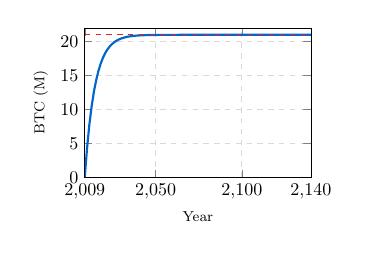
\begin{tikzpicture}[scale=0.65]
\begin{axis}[
    width=6cm, height=4.5cm,
    xlabel={\footnotesize Year},
    ylabel={\footnotesize BTC (M)},
    xmin=2009, xmax=2140,
    ymin=0, ymax=22,
    grid=major,
    grid style={dashed, gray!30},
    xtick={2009, 2050, 2100, 2140},
]
\addplot[very thick, dfblue, domain=2009:2140, samples=100]
    {21 * (1 - 2^(-(x-2009)/4))};
\addplot[dashed, dfred] coordinates {(2009,21) (2140,21)};
\end{axis}
\end{tikzpicture}

\footnotesize Asymptotically approaches 21M
\end{center}
\end{column}
\end{columns}

\bottomnote{Bitcoin maximalists: ``We already have one neutral, global money. Why do we need more?''}
\end{frame}

\begin{frame}{Bitcoin's Halving Mechanism}
\begin{block}{Definition: Halving}
The \textbf{halving} is a pre-programmed event where Bitcoin's block reward is cut in half every 210,000 blocks (approximately every 4 years).
\end{block}

\vspace{3mm}
\begin{center}
\begin{tabular}{c|c|c}
\toprule
\textbf{Halving} & \textbf{Year} & \textbf{Block Reward} \\
\midrule
Genesis & 2009 & 50 BTC \\
1st & 2012 & 25 BTC \\
2nd & 2016 & 12.5 BTC \\
3rd & 2020 & 6.25 BTC \\
4th & 2024 & 3.125 BTC \\
\bottomrule
\end{tabular}
\end{center}

\vspace{3mm}
\textbf{Why it matters:}
\begin{itemize}\compactlist
\item Creates predictable, decreasing inflation
\item Ensures 21M cap is never exceeded
\item Historically associated with price increases (supply shock)
\end{itemize}
\end{frame}

\begin{frame}{Ethereum: The World Computer Thesis}
\begin{columns}[T]
\begin{column}{0.55\textwidth}
\textbf{Core Properties}
\begin{itemize}\compactlist
\item \textbf{Smart contracts:} Self-executing code
\item \textbf{EVM:} Ethereum Virtual Machine
\item \textbf{Programmable:} Any logic possible
\item \textbf{Composable:} Contracts call contracts
\item \textbf{Tokens:} Create new assets easily
\end{itemize}

\vspace{3mm}
\textbf{The Narrative}
\begin{itemize}\compactlist
\item Platform for decentralized apps
\item ``DeFi'' -- finance without banks
\item NFTs, DAOs, and more
\item Base layer for Web3
\end{itemize}
\end{column}
\begin{column}{0.42\textwidth}
\begin{center}
\textbf{Ethereum Stack}

\vspace{2mm}
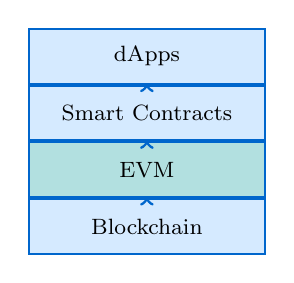
\begin{tikzpicture}[scale=0.8]
% EVM stack
\node[process, minimum width=3cm, minimum height=0.7cm] (l1) at (0,0) {\footnotesize dApps};
\node[process, minimum width=3cm, minimum height=0.7cm] (l2) at (0,-0.9) {\footnotesize Smart Contracts};
\node[process, minimum width=3cm, minimum height=0.7cm, fill=dfteal!30] (l3) at (0,-1.8) {\footnotesize EVM};
\node[process, minimum width=3cm, minimum height=0.7cm] (l4) at (0,-2.7) {\footnotesize Blockchain};

\draw[thick, dfblue, <->] (l1.south) -- (l2.north);
\draw[thick, dfblue, <->] (l2.south) -- (l3.north);
\draw[thick, dfblue, <->] (l3.south) -- (l4.north);
\end{tikzpicture}

\footnotesize Apps built on contracts on EVM\\
\footnotesize (EVM explained in detail next)
\end{center}
\end{column}
\end{columns}

\bottomnote{Ethereum enables ``programmable money'' -- money with built-in rules}
\end{frame}

\begin{frame}{Key Term: The Ethereum Virtual Machine (EVM)}
\begin{block}{Definition: EVM}
The \textbf{Ethereum Virtual Machine} is a runtime environment that executes smart contract code. Every Ethereum node runs the same EVM, ensuring consistent execution worldwide.
\end{block}

\vspace{3mm}
\begin{columns}[T]
\begin{column}{0.48\textwidth}
\textbf{How it Works}
\begin{enumerate}\compactlist
\item Developer writes contract (Solidity)
\item Code compiles to EVM bytecode
\item Bytecode deployed to blockchain
\item Every node can execute the code
\item Results are deterministic
\end{enumerate}
\end{column}
\begin{column}{0.48\textwidth}
\textbf{Key Properties}
\begin{itemize}\compactlist
\item \textbf{Deterministic:} Same input = same output
\item \textbf{Isolated:} Sandboxed execution
\item \textbf{Metered:} Gas limits computation
\item \textbf{Global:} Runs on all nodes
\end{itemize}
\end{column}
\end{columns}

\vspace{3mm}
\bottomnote{The EVM is like a global computer where everyone sees and verifies the same computation.}
\end{frame}

\begin{frame}{What Are Smart Contracts?}
\begin{columns}[T]
\begin{column}{0.48\textwidth}
\textbf{Traditional Contract}

\begin{enumerate}\compactlist
\item Legal document
\item Human interpretation
\item Court enforcement
\item (Maybe) execution
\end{enumerate}

\vspace{3mm}
Requires: lawyers, courts, trust
\end{column}
\begin{column}{0.48\textwidth}
\textbf{Smart Contract}

\begin{enumerate}\compactlist
\item Code on blockchain
\item Automatic execution
\item No intermediaries
\item Guaranteed outcome
\end{enumerate}

\vspace{3mm}
Requires: only the code
\end{column}
\end{columns}

\vspace{5mm}
\begin{block}{Definition: Smart Contract}
A smart contract is code stored on a blockchain that automatically executes when predetermined conditions are met.

\textbf{Key property:} Once deployed, the code cannot be changed. ``Code is law.''
\end{block}
\end{frame}

\begin{frame}{Smart Contract Example: Escrow}
\begin{columns}[T]
\begin{column}{0.48\textwidth}
\textbf{Traditional Escrow}
\begin{enumerate}\compactlist
\item Buyer sends money to escrow agent
\item Seller ships goods
\item Buyer confirms receipt
\item Escrow agent releases funds to seller
\end{enumerate}

\vspace{3mm}
\textbf{Problems:}
\begin{itemize}\compactlist
\item Trust the escrow agent
\item Agent takes a fee
\item Disputes are slow
\item Counterparty risk
\end{itemize}
\end{column}
\begin{column}{0.48\textwidth}
\textbf{Smart Contract Escrow}
\begin{enumerate}\compactlist
\item Buyer sends ETH to contract
\item Contract holds funds
\item Buyer calls \texttt{confirmReceipt()}
\item Contract automatically sends to seller
\end{enumerate}

\vspace{3mm}
\textbf{Advantages:}
\begin{itemize}\compactlist
\item Trust the code (auditable)
\item Minimal fees (just gas)
\item Instant execution
\item No counterparty risk
\end{itemize}
\end{column}
\end{columns}

\vspace{3mm}
\begin{center}
\fbox{\parbox{0.7\textwidth}{\centering
\textbf{Key insight:} Smart contracts replace trusted intermediaries with verified code.
}}
\end{center}
\end{frame}

\begin{frame}{Key Term: Gas}
\begin{block}{Definition: Gas}
\textbf{Gas} is the unit that measures computational work in Ethereum. Users pay gas fees (in ETH) to compensate validators for processing transactions.
\end{block}

\vspace{3mm}
\textbf{Why Gas Exists:}
\begin{enumerate}\compactlist
\item \textbf{Prevents infinite loops:} Turing-complete code could run forever
\item \textbf{Allocates resources:} Scarce block space needs rationing
\item \textbf{Compensates validators:} Payment for processing
\item \textbf{Spam prevention:} Makes attacks expensive
\end{enumerate}

\vspace{3mm}
\textbf{Gas Calculation:}
\begin{center}
\fbox{\textbf{Transaction Fee} = Gas Used $\times$ Gas Price}
\end{center}

\vspace{2mm}
\textbf{Example:} Simple ETH transfer uses $\sim$21,000 gas. At 50 gwei/gas = 0.00105 ETH fee.

\bottomnote{Bitcoin doesn't need gas because its scripting is intentionally limited and cannot loop forever.}
\end{frame}

\begin{frame}{What ``Programmable Money'' Enables}
\begin{columns}[T]
\begin{column}{0.32\textwidth}
\textbf{DeFi}
\begin{itemize}\compactlist
\item Lending/borrowing
\item Decentralized exchanges
\item Yield farming
\item Derivatives
\end{itemize}
\end{column}
\begin{column}{0.32\textwidth}
\textbf{NFTs/Tokens}
\begin{itemize}\compactlist
\item Digital ownership
\item Tokenized assets
\item Loyalty programs
\item Gaming items
\end{itemize}
\end{column}
\begin{column}{0.32\textwidth}
\textbf{DAOs}
\begin{itemize}\compactlist
\item Decentralized governance
\item Treasury management
\item Collective ownership
\item Voting systems
\end{itemize}
\end{column}
\end{columns}

\vspace{5mm}
\begin{center}
All built on Ethereum's programmable foundation
\end{center}

\vspace{3mm}
\begin{block}{The Power of Composability}
Smart contracts can call other smart contracts. This means DeFi protocols can be combined like Lego blocks -- creating entirely new financial products.
\end{block}
\end{frame}

\begin{frame}{Key Terms: DeFi, NFT, DAO}
\begin{columns}[T]
\begin{column}{0.32\textwidth}
\begin{block}{DeFi}
\textbf{Decentralized Finance}

Financial services (lending, trading, insurance) built on smart contracts without traditional intermediaries like banks.
\end{block}
\end{column}
\begin{column}{0.32\textwidth}
\begin{block}{NFT}
\textbf{Non-Fungible Token}

A unique digital asset on the blockchain representing ownership of a specific item (art, collectibles, real estate).
\end{block}
\end{column}
\begin{column}{0.32\textwidth}
\begin{block}{DAO}
\textbf{Decentralized Autonomous Organization}

An organization governed by smart contract rules and token-holder voting, with no traditional management structure.
\end{block}
\end{column}
\end{columns}

\vspace{5mm}
\begin{center}
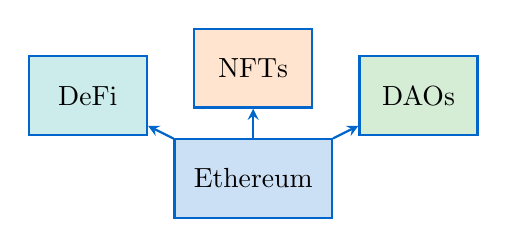
\begin{tikzpicture}[scale=0.7]
\node[process, minimum width=2cm, fill=dfblue!20] (eth) at (0,0) {Ethereum};
\node[process, minimum width=1.5cm, fill=dfteal!20] (defi) at (-3,1.5) {DeFi};
\node[process, minimum width=1.5cm, fill=dforange!20] (nft) at (0,2) {NFTs};
\node[process, minimum width=1.5cm, fill=dfgreen!20] (dao) at (3,1.5) {DAOs};

\draw[arrow] (eth) -- (defi);
\draw[arrow] (eth) -- (nft);
\draw[arrow] (eth) -- (dao);
\end{tikzpicture}
\end{center}
\end{frame}

\begin{frame}{The Tradeoff: Flexibility vs. Security}
\begin{columns}[T]
\begin{column}{0.48\textwidth}
\textbf{Bitcoin's Approach}
\begin{itemize}\compactlist
\item Limited scripting = fewer bugs
\item Simple = easier to secure
\item Ossification as a feature
\item ``If it ain't broke...''
\end{itemize}

\vspace{3mm}
\textbf{Security record:}
\begin{itemize}\compactlist
\item \textcolor{dfgreen}{Never been hacked}
\item No major protocol bugs
\item Predictable behavior
\item 15+ years of uptime
\end{itemize}
\end{column}
\begin{column}{0.48\textwidth}
\textbf{Ethereum's Approach}
\begin{itemize}\compactlist
\item Full programmability = more power
\item Complex = more attack surface
\item Continuous improvement
\item ``Move fast, fix things''
\end{itemize}

\vspace{3mm}
\textbf{Security record:}
\begin{itemize}\compactlist
\item \textcolor{dfred}{Many contract hacks}
\item The DAO hack (2016): \$60M
\item Ongoing exploits in DeFi
\item ``Code is law'' cuts both ways
\end{itemize}
\end{column}
\end{columns}

\vspace{3mm}
\begin{block}{The Fundamental Tradeoff}
More programmability = more capability = more things that can go wrong
\end{block}
\end{frame}

\begin{frame}{Case Study: The DAO Hack (2016)}
\begin{block}{What Happened}
The DAO was a smart contract that raised \$150M in ETH. A bug in the code allowed an attacker to drain \$60M.
\end{block}

\vspace{3mm}
\textbf{The Dilemma:}
\begin{itemize}\compactlist
\item The code executed exactly as written -- no protocol bug
\item ``Code is law'' -- should the theft stand?
\item But \$60M was stolen due to a coding error
\end{itemize}

\vspace{3mm}
\textbf{Ethereum's Response:}
\begin{itemize}\compactlist
\item Community voted to ``hard fork'' -- reverse the hack
\item Created two chains: Ethereum (ETH) and Ethereum Classic (ETC)
\item ETH: Reversed the hack | ETC: Kept the theft
\end{itemize}

\vspace{3mm}
\textbf{Lesson:} ``Code is law'' conflicts with ``humans make mistakes.'' Ethereum chose human intervention; Bitcoin's philosophy would not.
\end{frame}

\begin{frame}{Consensus: PoW vs. PoS}
\begin{center}
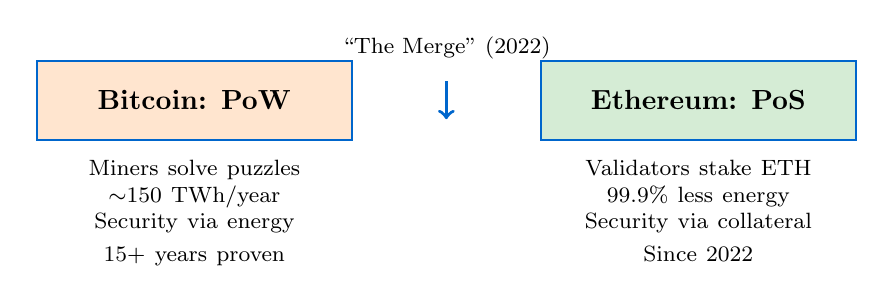
\begin{tikzpicture}[scale=0.8]
% Bitcoin PoW
\node[process, minimum width=4cm, fill=dforange!20] (btc) at (-4,0) {\textbf{Bitcoin: PoW}};
\node[anchor=north, text width=4cm, align=center] at (-4,-0.8) {
\footnotesize
Miners solve puzzles\\
$\sim$150 TWh/year\\
Security via energy\\
15+ years proven
};

% Ethereum PoS
\node[process, minimum width=4cm, fill=dfgreen!20] (eth) at (4,0) {\textbf{Ethereum: PoS}};
\node[anchor=north, text width=4cm, align=center] at (4,-0.8) {
\footnotesize
Validators stake ETH\\
99.9\% less energy\\
Security via collateral\\
Since 2022
};

% Arrow
\draw[very thick, ->, dfblue] (0,0.3) -- (0,-0.3);
\node[above] at (0,0.5) {\footnotesize ``The Merge'' (2022)};
\end{tikzpicture}
\end{center}

\vspace{5mm}
\begin{columns}[T]
\begin{column}{0.48\textwidth}
\textbf{Why Bitcoin keeps PoW:}
\begin{itemize}\compactlist
\item Proven security model
\item True external cost to attack
\item Conservative philosophy
\end{itemize}
\end{column}
\begin{column}{0.48\textwidth}
\textbf{Why Ethereum moved to PoS:}
\begin{itemize}\compactlist
\item Environmental concerns
\item Enables future scaling
\item Progressive philosophy
\end{itemize}
\end{column}
\end{columns}
\end{frame}

\begin{frame}{Market Positioning}
\begin{center}
\begin{tabular}{l|c|c|l}
\toprule
\textbf{Chain} & \textbf{Programmability} & \textbf{Market Cap} & \textbf{Niche} \\
\midrule
Bitcoin & Low & \#1 & Store of value \\
Ethereum & High & \#2 & Smart contract platform \\
Solana & High & \#5 & High-speed DeFi \\
Cardano & High & \#9 & Academic approach \\
\bottomrule
\end{tabular}
\end{center}

\vspace{5mm}
\textbf{Different chains, different niches:}
\begin{itemize}
\item Bitcoin: Store of value, ``digital gold'', settlement layer
\item Ethereum: Smart contract platform, DeFi hub
\item Other L1s: Compete on speed, cost, specific use cases
\end{itemize}

\vspace{3mm}
\textbf{Key insight:} It's not ``which chain wins'' -- it's ``which chain for which use case''
\end{frame}

\begin{frame}{Layer 2 Scaling Solutions}
\textbf{Problem:} Both Bitcoin ($\sim$7 TPS) and Ethereum ($\sim$15-30 TPS) are slow compared to Visa ($\sim$24,000 TPS).

\vspace{3mm}
\begin{columns}[T]
\begin{column}{0.48\textwidth}
\textbf{Bitcoin: Lightning Network}
\begin{itemize}\compactlist
\item Payment channels
\item Off-chain transactions
\item Instant, low fees
\item Settles to main chain
\item Focus: payments
\end{itemize}

\vspace{2mm}
\begin{center}
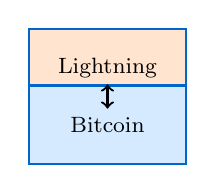
\begin{tikzpicture}[scale=0.6]
\node[process, minimum width=2cm, fill=dforange!20] (l2) at (0,0) {\footnotesize Lightning};
\node[process, minimum width=2cm] (l1) at (0,-1.2) {\footnotesize Bitcoin};
\draw[thick, <->] (l2) -- (l1);
\end{tikzpicture}
\end{center}
\end{column}
\begin{column}{0.48\textwidth}
\textbf{Ethereum: Rollups \& Sidechains}
\begin{itemize}\compactlist
\item Optimism, Arbitrum (rollups)
\item Polygon (sidechain)
\item Batch transactions
\item Submit proofs to L1
\item Focus: all applications
\end{itemize}

\vspace{2mm}
\begin{center}
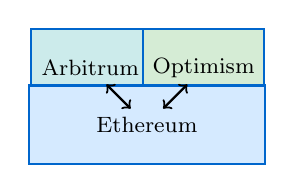
\begin{tikzpicture}[scale=0.6]
\node[process, minimum width=1.5cm, fill=dfteal!20] (r1) at (-1.2,0) {\footnotesize Arbitrum};
\node[process, minimum width=1.5cm, fill=dfgreen!20] (r2) at (1.2,0) {\footnotesize Optimism};
\node[process, minimum width=3cm] (l1) at (0,-1.2) {\footnotesize Ethereum};
\draw[thick, <->] (r1) -- (l1);
\draw[thick, <->] (r2) -- (l1);
\end{tikzpicture}
\end{center}
\end{column}
\end{columns}
\end{frame}

\begin{frame}{Development Philosophy Comparison}
\begin{center}
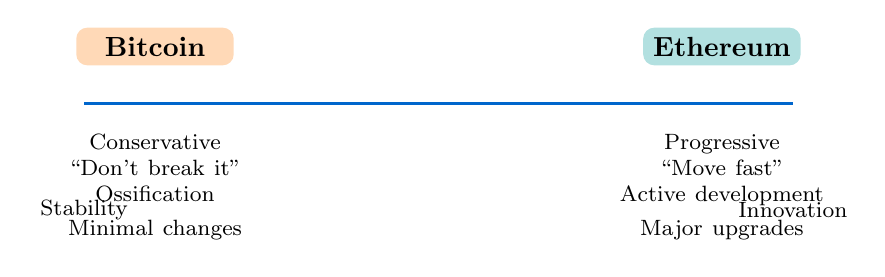
\begin{tikzpicture}[scale=0.9]
% Spectrum line
\draw[very thick, dfblue] (-5,0) -- (5,0);

% Bitcoin side
\node[fill=dforange!30, rounded corners, minimum width=2cm] at (-4,0.8) {\textbf{Bitcoin}};
\node[anchor=north, text width=3cm, align=center] at (-4,-0.3) {
\footnotesize
Conservative\\
``Don't break it''\\
Ossification\\
Minimal changes
};

% Ethereum side
\node[fill=dfteal!30, rounded corners, minimum width=2cm] at (4,0.8) {\textbf{Ethereum}};
\node[anchor=north, text width=3cm, align=center] at (4,-0.3) {
\footnotesize
Progressive\\
``Move fast''\\
Active development\\
Major upgrades
};

% Labels
\node at (-5,-1.5) {\footnotesize Stability};
\node at (5,-1.5) {\footnotesize Innovation};
\end{tikzpicture}
\end{center}

\vspace{5mm}
\begin{columns}[T]
\begin{column}{0.48\textwidth}
\textbf{Bitcoin Changes:}
\begin{itemize}\compactlist
\item SegWit (2017): Scaling fix
\item Taproot (2021): Privacy + smart contracts
\item Years of debate for each change
\end{itemize}
\end{column}
\begin{column}{0.48\textwidth}
\textbf{Ethereum Changes:}
\begin{itemize}\compactlist
\item EIP-1559 (2021): Fee mechanism
\item The Merge (2022): PoW to PoS
\item Dencun (2024): Blob transactions
\item Regular hard forks
\end{itemize}
\end{column}
\end{columns}
\end{frame}

% =============================================================================
% SLIDES 25-28: Additional Content (no notebook)
% =============================================================================
\begin{frame}{Case Study: Bitcoin as Treasury Asset}
\textbf{MicroStrategy's Bitcoin Strategy}

\vspace{3mm}
\begin{itemize}
\item CEO Michael Saylor began buying Bitcoin in 2020
\item Rationale: Protect treasury from dollar inflation
\item Holdings: 200,000+ BTC (as of 2024)
\item Treats Bitcoin as ``digital gold'' for corporate reserves
\end{itemize}

\vspace{3mm}
\textbf{Why Bitcoin (not Ethereum)?}
\begin{enumerate}\compactlist
\item Fixed supply -- predictable scarcity
\item No protocol changes -- long-term stability
\item Simpler to value -- pure store of value thesis
\item Regulatory clarity -- treated as commodity in US
\end{enumerate}

\vspace{3mm}
\begin{block}{Implication}
Bitcoin's conservative design makes it attractive for entities seeking predictable, long-term value storage.
\end{block}
\end{frame}

\begin{frame}{Case Study: Ethereum as DeFi Infrastructure}
\textbf{Uniswap: Decentralized Exchange}

\vspace{3mm}
\begin{itemize}
\item Launched 2018 on Ethereum
\item No order book -- uses automated market makers (AMM)
\item Over \$1 trillion in cumulative trading volume
\item Governance by UNI token holders
\end{itemize}

\vspace{3mm}
\textbf{Why Ethereum (not Bitcoin)?}
\begin{enumerate}\compactlist
\item Requires smart contracts -- not possible on Bitcoin
\item Needs token creation -- ERC-20 standard
\item Composability -- integrates with other DeFi protocols
\item EVM ecosystem -- developers, tools, infrastructure
\end{enumerate}

\vspace{3mm}
\begin{block}{Implication}
Ethereum's programmability enables financial applications impossible on Bitcoin, but with added complexity and risk.
\end{block}
\end{frame}

\begin{frame}{Case Study: Cross-Chain Bridges}
\textbf{Problem:} Users want Bitcoin's store of value + Ethereum's DeFi

\vspace{3mm}
\textbf{Solution: Wrapped Bitcoin (WBTC)}
\begin{itemize}
\item ERC-20 token on Ethereum backed 1:1 by Bitcoin
\item Allows BTC holders to participate in DeFi
\item Over \$5 billion in circulation
\end{itemize}

\vspace{3mm}
\begin{center}
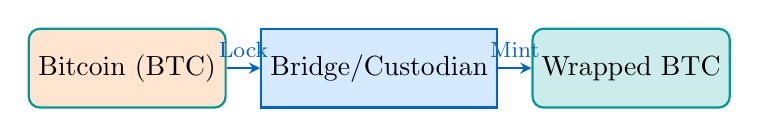
\begin{tikzpicture}[scale=0.8]
\node[blockchain, fill=dforange!20] (btc) at (0,0) {Bitcoin (BTC)};
\node[process, minimum width=2cm] (bridge) at (4,0) {Bridge/Custodian};
\node[blockchain, fill=dfteal!20] (wbtc) at (8,0) {Wrapped BTC};

\draw[arrow] (btc) -- node[above]{\footnotesize Lock} (bridge);
\draw[arrow] (bridge) -- node[above]{\footnotesize Mint} (wbtc);
\end{tikzpicture}
\end{center}

\vspace{3mm}
\textbf{Risks:}
\begin{itemize}\compactlist
\item Custodial risk -- trust the bridge operator
\item Bridge hacks -- over \$2B stolen from bridges (2021-2023)
\item Regulatory uncertainty
\end{itemize}
\end{frame}

\begin{frame}{Regulatory Landscape: Bitcoin vs. Ethereum}
\begin{columns}[T]
\begin{column}{0.48\textwidth}
\textbf{Bitcoin: Generally Clearer}
\begin{itemize}\compactlist
\item US: Treated as commodity (CFTC)
\item No pre-mine, no foundation
\item Decentralized from day one
\item Spot ETFs approved (2024)
\end{itemize}

\vspace{3mm}
\textcolor{dfgreen}{Lower regulatory risk}
\end{column}
\begin{column}{0.48\textwidth}
\textbf{Ethereum: More Complex}
\begin{itemize}\compactlist
\item Had ICO (initial coin offering)
\item Ethereum Foundation exists
\item Proof of Stake = ``staking rewards''
\item SEC scrutiny on classification
\end{itemize}

\vspace{3mm}
\textcolor{dfred}{Higher regulatory uncertainty}
\end{column}
\end{columns}

\vspace{5mm}
\begin{block}{Key Question}
Is ETH a security or a commodity? The answer affects exchanges, staking services, and DeFi protocols. Bitcoin's simpler design avoids this ambiguity.
\end{block}
\end{frame}

% =============================================================================
% SLIDES 29-30: Discussion/Application
% =============================================================================
\begin{frame}{Discussion Questions}
\begin{enumerate}
\item \textbf{Store of value vs. programmability:} Can Ethereum also be ``sound money''? Can Bitcoin add smart contracts?

\vspace{3mm}
\item \textbf{The DAO hack:} Ethereum's response (hard fork to reverse the hack) violated ``code is law.'' Was this the right call?

\vspace{3mm}
\item \textbf{Energy debate:} Bitcoin's PoW energy use is criticized, but it's also what makes it secure. Ethereum moved to PoS -- did it sacrifice anything?

\vspace{3mm}
\item \textbf{Maximalism:} Many believe only one blockchain will ``win.'' Others see room for many. What's your view?

\vspace{3mm}
\item \textbf{Regulation:} How might different design philosophies affect regulatory treatment? Is ETH a security?
\end{enumerate}
\end{frame}

\begin{frame}{Application: Choosing a Platform}
\textbf{Scenario:} You're advising a startup on blockchain strategy.

\vspace{3mm}
\begin{center}
\begin{tabular}{l|c|c}
\toprule
\textbf{Use Case} & \textbf{Best Fit} & \textbf{Why} \\
\midrule
Corporate treasury reserve & Bitcoin & Fixed supply, stability \\
Decentralized lending app & Ethereum & Smart contracts \\
Cross-border remittances & Either/L2 & Speed vs. security tradeoff \\
Tokenized real estate & Ethereum & Token standards \\
Long-term savings (10+ years) & Bitcoin & Conservative, proven \\
NFT marketplace & Ethereum & ERC-721 standard \\
\bottomrule
\end{tabular}
\end{center}

\vspace{5mm}
\begin{block}{Key Takeaway}
The right platform depends on your specific needs. Understanding both philosophies helps you make informed decisions.
\end{block}
\end{frame}

% =============================================================================
% SLIDE 31: Executive Summary
% =============================================================================
\begin{frame}{Executive Summary}
\begin{enumerate}
\item \textbf{Different Goals:} Bitcoin = sound money (store of value); Ethereum = world computer (programmable platform)

\vspace{3mm}
\item \textbf{Key Technical Difference:} Bitcoin Script is limited by design; Ethereum's EVM is Turing-complete

\vspace{3mm}
\item \textbf{The Tradeoff:} More programmability means more capability but also more attack surface

\vspace{3mm}
\item \textbf{Not Competitors:} They serve different use cases and can coexist

\vspace{3mm}
\item \textbf{Both Face Scaling Challenges:} Layer 2 solutions (Lightning, Rollups) address throughput limits
\end{enumerate}

\vspace{5mm}
\begin{center}
\fbox{\parbox{0.8\textwidth}{\centering
\textbf{Bottom Line:} Understanding both platforms' design philosophies is essential for navigating digital finance.
}}
\end{center}
\end{frame}

% =============================================================================
% SLIDE 32: Concept Map
% =============================================================================
\begin{frame}{Concept Map: Architecture Comparison}
\begin{center}
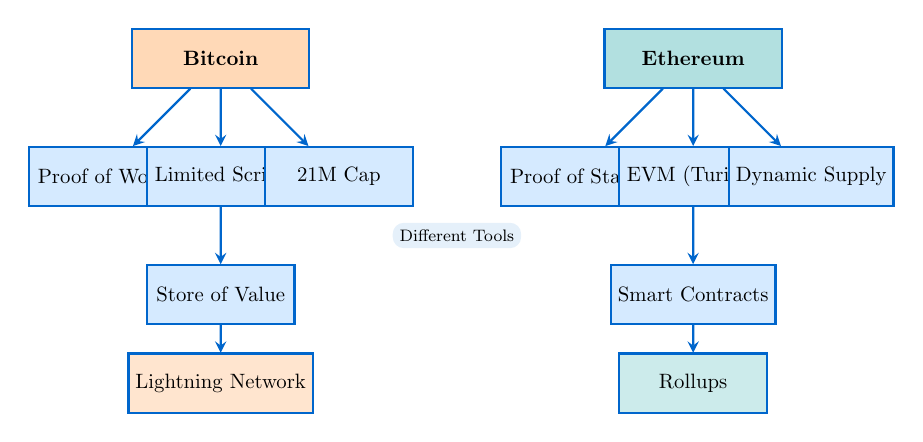
\begin{tikzpicture}[scale=0.75, transform shape]
% Bitcoin side
\node[process, minimum width=3cm, fill=dforange!30] (btc) at (-4,3) {\textbf{Bitcoin}};
\node[process, minimum width=2.5cm] (btc_pow) at (-6,1) {Proof of Work};
\node[process, minimum width=2.5cm] (btc_script) at (-4,1) {Limited Script};
\node[process, minimum width=2.5cm] (btc_supply) at (-2,1) {21M Cap};
\node[process, minimum width=2.5cm] (btc_use) at (-4,-1) {Store of Value};
\node[process, minimum width=2.5cm, fill=dforange!20] (btc_l2) at (-4,-2.5) {Lightning Network};

\draw[arrow] (btc) -- (btc_pow);
\draw[arrow] (btc) -- (btc_script);
\draw[arrow] (btc) -- (btc_supply);
\draw[arrow] (btc_script) -- (btc_use);
\draw[arrow] (btc_use) -- (btc_l2);

% Ethereum side
\node[process, minimum width=3cm, fill=dfteal!30] (eth) at (4,3) {\textbf{Ethereum}};
\node[process, minimum width=2.5cm] (eth_pos) at (2,1) {Proof of Stake};
\node[process, minimum width=2.5cm] (eth_evm) at (4,1) {EVM (Turing)};
\node[process, minimum width=2.5cm] (eth_supply) at (6,1) {Dynamic Supply};
\node[process, minimum width=2.5cm] (eth_use) at (4,-1) {Smart Contracts};
\node[process, minimum width=2.5cm, fill=dfteal!20] (eth_l2) at (4,-2.5) {Rollups};

\draw[arrow] (eth) -- (eth_pos);
\draw[arrow] (eth) -- (eth_evm);
\draw[arrow] (eth) -- (eth_supply);
\draw[arrow] (eth_evm) -- (eth_use);
\draw[arrow] (eth_use) -- (eth_l2);

% Center comparison
\node[fill=dfblue!10, rounded corners] at (0,0) {\footnotesize Different Tools};
\end{tikzpicture}
\end{center}
\end{frame}

% =============================================================================
% SLIDES 33-34: Key Terms & Definitions
% =============================================================================
\begin{frame}{Key Terms \& Definitions (1/2)}
\begin{description}
\item[Turing-Complete] A system that can compute anything computable; has the power of a general-purpose computer. Ethereum's EVM is Turing-complete; Bitcoin Script is not.

\vspace{2mm}
\item[Smart Contract] Code stored on a blockchain that automatically executes when conditions are met. Immutable once deployed (``code is law'').

\vspace{2mm}
\item[EVM] Ethereum Virtual Machine -- the runtime environment that executes smart contract code on every Ethereum node.

\vspace{2mm}
\item[Gas] The unit measuring computational work in Ethereum. Users pay gas fees to compensate validators and prevent infinite loops.

\vspace{2mm}
\item[Halving] Bitcoin's pre-programmed event where block rewards are cut in half every 210,000 blocks, ensuring the 21M supply cap.
\end{description}
\end{frame}

\begin{frame}{Key Terms \& Definitions (2/2)}
\begin{description}
\item[DeFi] Decentralized Finance -- financial services (lending, trading, insurance) built on smart contracts without traditional intermediaries.

\vspace{2mm}
\item[NFT] Non-Fungible Token -- a unique digital asset representing ownership of a specific item on the blockchain.

\vspace{2mm}
\item[DAO] Decentralized Autonomous Organization -- an organization governed by smart contract rules and token-holder voting.

\vspace{2mm}
\item[Layer 2] Solutions built on top of a blockchain (Layer 1) to increase transaction throughput while inheriting the base layer's security.

\vspace{2mm}
\item[The Merge] Ethereum's September 2022 transition from Proof of Work to Proof of Stake, reducing energy consumption by 99.9\%.
\end{description}
\end{frame}

% =============================================================================
% SLIDE 35: Common Misconceptions
% =============================================================================
\begin{frame}{Common Misconceptions}
\begin{columns}[T]
\begin{column}{0.48\textwidth}
\textbf{\textcolor{dfred}{Myth}}
\end{column}
\begin{column}{0.48\textwidth}
\textbf{\textcolor{dfgreen}{Reality}}
\end{column}
\end{columns}

\vspace{3mm}
\hrule
\vspace{3mm}

\textbf{``Bitcoin and Ethereum are direct competitors''}\\
\textcolor{dfgreen}{They solve different problems: Bitcoin = sound money; Ethereum = programmable platform}

\vspace{3mm}
\hrule
\vspace{3mm}

\textbf{``Ethereum is just a faster Bitcoin''}\\
\textcolor{dfgreen}{Ethereum's speed is secondary to its programmability. Bitcoin is intentionally slower for security.}

\vspace{3mm}
\hrule
\vspace{3mm}

\textbf{``Smart contracts can do anything''}\\
\textcolor{dfgreen}{They can only access on-chain data. Real-world data requires ``oracles'' (trusted data feeds).}

\vspace{3mm}
\hrule
\vspace{3mm}

\textbf{``Proof of Stake is always better than Proof of Work''}\\
\textcolor{dfgreen}{Each has tradeoffs. PoW provides external security cost; PoS is more energy efficient but newer.}
\end{frame}

% =============================================================================
% SLIDE 36: Industry Perspective
% =============================================================================
\begin{frame}{Industry Perspective: Who Uses What?}
\begin{center}
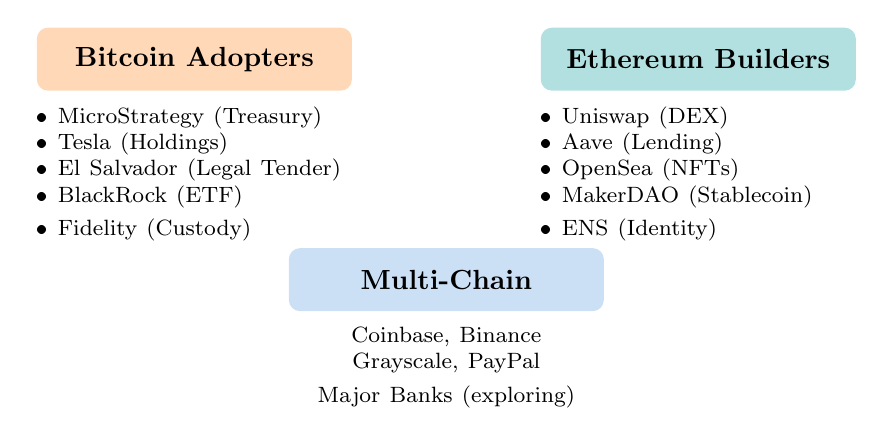
\begin{tikzpicture}[scale=0.8]
% Bitcoin column
\node[fill=dforange!30, rounded corners, minimum width=4cm, minimum height=0.8cm] at (-4,3) {\textbf{Bitcoin Adopters}};
\node[anchor=north, text width=4cm, align=left] at (-4,2.4) {
\footnotesize
\textbullet\ MicroStrategy (Treasury)\\
\textbullet\ Tesla (Holdings)\\
\textbullet\ El Salvador (Legal Tender)\\
\textbullet\ BlackRock (ETF)\\
\textbullet\ Fidelity (Custody)
};

% Ethereum column
\node[fill=dfteal!30, rounded corners, minimum width=4cm, minimum height=0.8cm] at (4,3) {\textbf{Ethereum Builders}};
\node[anchor=north, text width=4cm, align=left] at (4,2.4) {
\footnotesize
\textbullet\ Uniswap (DEX)\\
\textbullet\ Aave (Lending)\\
\textbullet\ OpenSea (NFTs)\\
\textbullet\ MakerDAO (Stablecoin)\\
\textbullet\ ENS (Identity)
};

% Both column
\node[fill=dfblue!20, rounded corners, minimum width=4cm, minimum height=0.8cm] at (0,-0.5) {\textbf{Multi-Chain}};
\node[anchor=north, text width=4cm, align=center] at (0,-1.1) {
\footnotesize
Coinbase, Binance\\
Grayscale, PayPal\\
Major Banks (exploring)
};
\end{tikzpicture}
\end{center}

\vspace{3mm}
\begin{block}{Pattern}
Institutions seeking \textbf{store of value} gravitate to Bitcoin.\\
Builders creating \textbf{applications} build on Ethereum.
\end{block}
\end{frame}

% =============================================================================
% SLIDES 37-38: Self-Assessment Questions
% =============================================================================
\begin{frame}{Self-Assessment Question 1}
\textbf{Q3: What is the main difference between Bitcoin Script and Ethereum's EVM?}

\vspace{3mm}
\begin{enumerate}[A)]
\item Bitcoin Script is faster than the EVM
\item Bitcoin Script is limited and not Turing-complete, while the EVM is Turing-complete
\item The EVM can only handle simple transactions
\item Bitcoin Script uses more gas than the EVM
\end{enumerate}

\vspace{5mm}
\pause
\textbf{Answer: B}

\vspace{2mm}
Bitcoin Script is intentionally limited and not Turing-complete -- it can answer simple yes/no questions like ``Is this a valid payment?'' The Ethereum Virtual Machine is Turing-complete, meaning it can run any computable program. Think of it as Bitcoin's simple calculator vs. Ethereum's full computer. This reflects their design philosophies: Bitcoin prioritizes security through simplicity; Ethereum prioritizes programmability.
\end{frame}

\begin{frame}{Self-Assessment Questions 2-3}
\textbf{Q11: How does Bitcoin's approach to changes differ from Ethereum's?}
\begin{enumerate}[A)]
\item Bitcoin has no way to make protocol changes
\item Bitcoin follows ``don't break what works''; Ethereum follows ``move fast, iterate''
\item Ethereum never makes protocol changes
\item Both make changes at exactly the same rate
\end{enumerate}

\textbf{Answer: B} -- Bitcoin is conservative; Ethereum is progressive.

\vspace{5mm}
\hrule
\vspace{3mm}

\textbf{Q19: What is the key tradeoff between Bitcoin's limited scripting and Ethereum's Turing-completeness?}
\begin{enumerate}[A)]
\item Bitcoin is faster than Ethereum
\item Bitcoin's simplicity provides fewer attack vectors; Ethereum's complexity enables more capabilities but more potential bugs
\item Ethereum cannot process simple payments
\item Bitcoin has no tradeoffs
\end{enumerate}

\textbf{Answer: B} -- More programmability = more capability = more attack surface.
\end{frame}

% =============================================================================
% SLIDE 38: What's Next
% =============================================================================
\begin{frame}{What's Next: Day 4}
\begin{center}
\textbf{\Large Programmable Finance}\\[3mm]
\textit{Smart Contracts, DeFi, and Tokenization}
\end{center}

\vspace{5mm}
\begin{itemize}
\item How smart contracts enable DeFi protocols
\item Lending, borrowing, and trading without intermediaries
\item Tokenization: bridging traditional and crypto finance
\item Real-world asset tokenization
\item Risks and opportunities in DeFi
\end{itemize}

\vspace{5mm}
\begin{center}
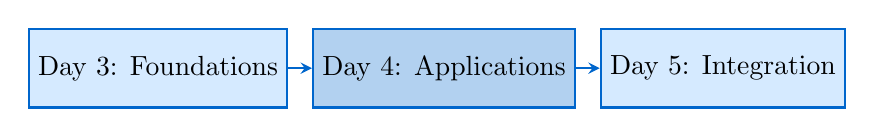
\begin{tikzpicture}
\node[process, minimum width=3cm] (d3) {Day 3: Foundations};
\node[process, minimum width=3cm, right=0.3cm of d3, fill=dfblue!30] (d4) {Day 4: Applications};
\node[process, minimum width=3cm, right=0.3cm of d4] (d5) {Day 5: Integration};

\draw[arrow] (d3) -- (d4);
\draw[arrow] (d4) -- (d5);
\end{tikzpicture}
\end{center}
\end{frame}

% =============================================================================
% SLIDE 39: Resources
% =============================================================================
\begin{frame}{Resources for Further Learning}
\textbf{Bitcoin}
\begin{itemize}\compactlist
\item Bitcoin Whitepaper: \url{bitcoin.org/bitcoin.pdf}
\item ``Mastering Bitcoin'' by Andreas Antonopoulos
\item Bitcoin Wiki: \url{en.bitcoin.it}
\end{itemize}

\vspace{3mm}
\textbf{Ethereum}
\begin{itemize}\compactlist
\item Ethereum Whitepaper: \url{ethereum.org/whitepaper}
\item ``Mastering Ethereum'' by Antonopoulos \& Wood
\item Ethereum Documentation: \url{ethereum.org/developers}
\end{itemize}

\vspace{3mm}
\textbf{Comparison \& Analysis}
\begin{itemize}\compactlist
\item CoinMetrics: On-chain data and research
\item Messari: Crypto asset intelligence
\item Glassnode: Bitcoin-focused analytics
\end{itemize}

\vspace{3mm}
\bottomnote{Remember: Focus on understanding the ``why'' behind design decisions, not just the ``what.''}
\end{frame}

% =============================================================================
% SLIDE 40: Questions?
% =============================================================================
\begin{frame}
\begin{center}
\vspace{1cm}
{\Huge Questions?}

\vspace{1.5cm}
\textbf{Topic 3.4: Bitcoin vs. Ethereum}\\[3mm]
Two Design Philosophies

\vspace{1cm}
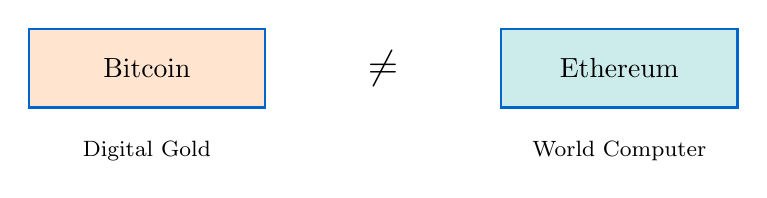
\begin{tikzpicture}
\node[process, minimum width=3cm, fill=dforange!20] (btc) at (-3,0) {Bitcoin};
\node[process, minimum width=3cm, fill=dfteal!20] (eth) at (3,0) {Ethereum};
\node at (0,0) {\Large $\neq$};

\node[below] at (-3,-0.8) {\footnotesize Digital Gold};
\node[below] at (3,-0.8) {\footnotesize World Computer};
\end{tikzpicture}

\vspace{1cm}
\textcolor{dfgray}{\small Joerg Osterrieder | Digital Finance | 2025}
\end{center}
\end{frame}

\end{document}
